% Created 2024-12-09 pon 19:44
% Intended LaTeX compiler: pdflatex
\documentclass[11pt]{article}
\usepackage[utf8]{inputenc}
\usepackage[T1]{fontenc}
\usepackage{graphicx}
\usepackage{longtable}
\usepackage{wrapfig}
\usepackage{rotating}
\usepackage[normalem]{ulem}
\usepackage{amsmath}
\usepackage{amssymb}
\usepackage{capt-of}
\usepackage{hyperref}
\usepackage[a4paper, margin=1.2in]{geometry}
\hypersetup{colorlinks=true,linkcolor=black}
\author{Piotr Jabłoński (325163) i Paweł Wysocki (325248)}
\date{Grudzień 2024}
\title{Dokumentacja wstepna projektu z UMA}
\hypersetup{
 pdfauthor={Piotr Jabłoński (325163) i Paweł Wysocki (325248)},
 pdftitle={Dokumentacja wstepna projektu z UMA},
 pdfkeywords={},
 pdfsubject={},
 pdfcreator={Emacs 29.4 (Org mode 9.7.11)}, 
 pdflang={Polish}}
\begin{document}

\maketitle
\tableofcontents

\pagebreak
\section{Temat projektu}
\label{sec:org004bb5c}
Celem naszego projektu jest implementacja algorytmu konstruującego drzewo klasyfikujące z wyborem testu przy pomocy ruletki.
\section{Opis problemu}
\label{sec:org19cc40d}

\subsection{Drzewo klasyfikacyjne}
\label{sec:orgdbf1c0f}
Drzewo klasyfikacyjne to relatywnie prosty model uczenia maszynowego. Polega on na konstrukcji drzewa binarnego gdzie:
\begin{itemize}
\item węzeł - atrybut, na podstawie którego dzielimy klasy na podzbiory. Tak zwany "test"
\item liść - klasa lub predykcja klasy
\end{itemize}
Jest to w pewnym sensie jedna wielka "if-else" instrukcja, z tą różnicą że wybór testu dla dodawanego węzłu odbywa się automatycznie. Najlepszy atrybut wybieramy na podstawie największego \textbf{zysku informacji} (Information Gain) dla tego atrybutu.

W tym zadaniu izolujemy dane do momentu, gdzie wszystkie dane należą do tej samej klasy (dane jednorodne). Im wybierzemy lepszy test do podziału danych, tym precyzyjniej i ogólniej nasze drzewo się będzie zachowywało. Naszym celem jest więc znalezienie takiego testu, aby maksymalnie zmiejszyć entropię całego zbioru.

\begin{center}
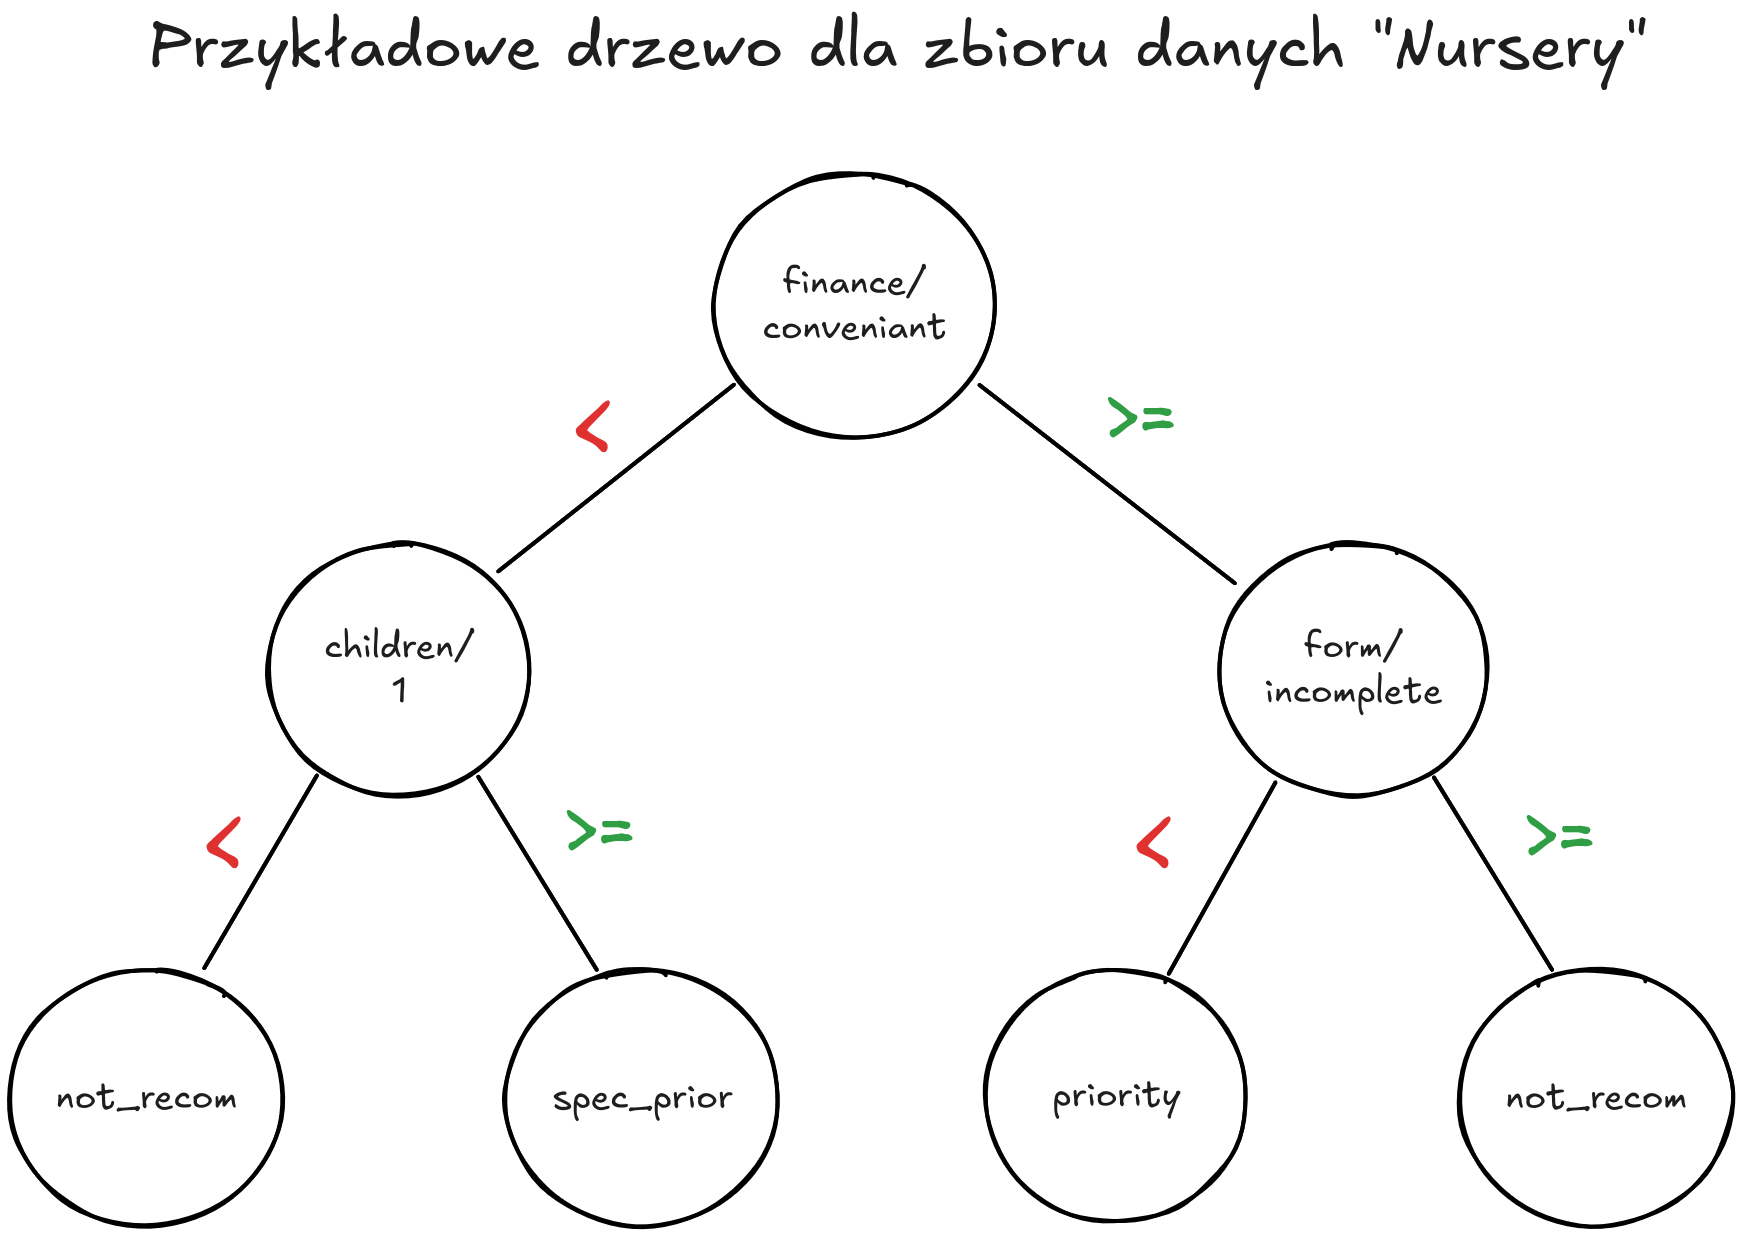
\includegraphics[width=.9\linewidth]{./images/example-nursery-tree.png}
\end{center}

\pagebreak
\subsection{Ruletka}
\label{sec:org67ac858}
Zwykle drzewa decyzyjne są zachłanne, tzn. wybierają ten test, który ma największą jakość. Takie podejście jest proste w realizacji oraz bardzo efektywne, natomiast takie drzewo jest bardzo łatwo przeuczyć. W naszym przypadku selekcja testu odbędzie się ruletkowo:
\[
        P(a_i) = \frac{IG(a_i)}{\sum_i^n{IG(a_j)}}
\]
gdzie
\begin{itemize}
\item P(a\textsubscript{i}) - prawdopodobieństwo wybrania atrybutu a\textsubscript{i}
\item IG(a\textsubscript{i}) - zysk informacji dla atrybutu a\textsubscript{i}
\item n - ilość atrybutów
\end{itemize}
Takie podejście sprawia, że prawdopodobieństwo wybrania testu dla atrybutu a\textsubscript{i} jest wprost-proporcjonalne do zysku informacji, dzięki czemu drzewa powinny mieć miejszą podatność na przeuczenie.
\subsection{Algorytmy}
\label{sec:org4909e92}
Żeby skonstruować drzewo klasyfikacyjne potrzebujemy 3 algorytmów:
\begin{itemize}
\item Algorytm budowania drzewa
\item Algorytm wyboru testu z ruletką
\item Algorytm obliczania zysku informacji (\textbf{IG})
\end{itemize}
Opracowaliśmy pseudokod w języku Python-podobnym, żeby lepiej zwizualizować nasz tok myślenia:
\subsubsection{Algorytm budowania drzewa}
\label{sec:org8d16fe2}
\begin{verbatim}
def build_tree(attrs, data, classes, max_depth) -> DecisionTree:
    if max_depth == 0 or len(attrs) == 0:
        return most_common(attrs)

    tree = DecisionTree()

    # przeprowadzamy test z ruletką
    tree.attr, tree.threshold = test(attrs, data, classes)
    new_attr = attrs - tree.attr

    # dzielimy dane na postawie testu
    left_data, right_data = [...]
    tree.left = build_tree(new_attr, left_data, classes, max_depth - 1)
    tree.right = build_tree(new_attr, right_data, classes, max_depth - 1)

    return tree
\end{verbatim}
\subsubsection{Algorytm wyboru testu z ruletką}
\label{sec:orge6811b9}
\begin{verbatim}
def test(attrs, data, classes):
    IGs = []
    for a in attrs:
        for c in classes:
            IQs.append(IQ(a, data, classes, threshold=c))

    # ruletkowy wybór zysku informacji
    total = sum(IQs); running_total = 0; p = randint(0, total)
    for iq in IQs:
        running_total += iq
        if running_total >= p:
            return iq
\end{verbatim}
\subsubsection{Algorytm obliczania zysku informacji (\textbf{IG})}
\label{sec:org5372fdc}
Informacja to tak naprawdę różnica entropi węzła nadrzędnego i średniej ważonej entropii węzła potomnego. Im większy zysk informacji, tym bardziej zmiejszyliśmy entropię w danych - tym dane stają się czystrze.
\[
        IQ(S, a) = H(S) - \sum_{v \in vals(a)}{\frac{|Sv|}{|S|} \cdot H(Sv)}
\]
gdzie
\begin{itemize}
\item \(S\) - podzbiór danych
\item \(Sv\) - podzbiór danych po dzieleniu przez atrybut \(a\)
\item entropia \(H(S) = \sum_{i=1}{c} - p_i \cdot \log_2{p_i}\)
\end{itemize}
\section{Plan eksperymentów}
\label{sec:orgba831bb}
Aby przeprować odpowienie testy statystyczne postanowiliśmy przeprowadzić eksperymenty na wielu różnych zbiorach danych oraz porównać uzyskane wyniki do klasyfikatora \href{https://scikit-learn.org/stable/modules/generated/sklearn.tree.DecisionTreeClassifier.html\#decisiontreeclassifier}{DecisionTreeClassifer} z pakietu naukowego \href{https://scikit-learn.org}{scikit-learn}.

Macież błędów (tablica pomyłek) posłuży nam do zwizualizowania i zweryfikowania skuteczności klasyfikacji. Będziemy skupiać się na miarach: \textbf{PPV}, \textbf{Recall} i \textbf{F1}.

\pagebreak
\section{Zbiory danych}
\label{sec:org34135ba}
Przygotowaliśmy 4 zbiory danych, na których będziemy prowadzić eksperymenty.
\subsection{\href{https://www.kaggle.com/datasets/uciml/red-wine-quality-cortez-et-al-2009/data}{Red Wine Quality}}
\label{sec:orge712876}
Zawiera 11 fizykochemicznych atrybutów win:
\begin{enumerate}
\item Kwasowość stała
\item Kwasowość wulkaniczna
\item Kwas cytrynowy
\item Cukier pozostały
\item Chloridy
\item Dwutlenek siarki wolny
\item Dwutlenek siarki całkowity
\item Gęstość
\item pH
\item Siarczanaty
\item Procent alkoholu
\end{enumerate}
Zadanie klasyfikacji:
\begin{itemize}
\item Jakość wina w skali całkowitoliczbowej (1-10)
\end{itemize}
\subsection{\href{https://www.kaggle.com/datasets/taweilo/loan-approval-classification-data}{Loan Approval Classification}}
\label{sec:org43de68f}
Zawiera 9 atrybutów o osobie składającej wniosek o pożyczkę oraz 4 atrybuty o samej pożyczce - łącznie 13 atrybutów, na podstawie których należy zklasyfikować stan wniosku (zaakceptowany bądź odrzucony). Atrybuty:
\begin{enumerate}
\item Wiek
\item Płeć
\item Edukacja
\item Dochód roczny
\item Ilość lat doświadczenia zawodowego
\item Stan posiadania domu (wynajem, na własność, hipoteka)
\item Kwota pożyczki
\item Cel pożyczki
\item Oprocentowanie pożyczki
\item Wysokość wypożyczenia w relacji do dochodu rocznego (\%)
\item Zdolność kredytowa
\item Długość historii kredytowej w latach
\item Indikator wcześniejszych niespłaconych wypożyczeń
\end{enumerate}
Zadanie klasyfikacji:
\begin{itemize}
\item Akceptacja wniosku o pożyczkę (prawda/fałsz)
\end{itemize}
\subsection{\href{https://www.kaggle.com/datasets/nimapourmoradi/nursery}{Nursery}}
\label{sec:org0f4e062}
Zawiera 8 atrybutów dotyczących rodziny:
\begin{enumerate}
\item Zawód rodziców
\item Przedszkole dziecka
\item Struktura rodziny
\item Ilość dzieci
\item Warunki zamieszkania
\item Finansowa sytuacja
\item Społeczna sytuacja
\item Zdrowotna sytuacja
\end{enumerate}
Zadanie klasyfikacji:
\begin{itemize}
\item Ocena aplikacji do przedszkola (ocena stanu zdrowia rodziny)
\end{itemize}
\subsection{\href{https://www.kaggle.com/datasets/valakhorasani/mobile-device-usage-and-user-behavior-dataset}{Mobile Device Usage and User Behavior}}
\label{sec:org2f897e3}
\begin{enumerate}
\item Id użytkownika
\item Model urządzenia
\item System operacyjny
\item Czas używania aplikacji
\item SOT (Screen On Time)
\item Codzienne zużycie baterii (mAh)
\item Liczba zainstalowanych aplikacji
\item Codzienne zużycie danych
\item Wiek
\item Płeć (M/K)
\end{enumerate}
Zadanie klasyfikacji:
\begin{itemize}
\item Ocena zachowania użytkownika (od lekkiego do ekstremalnego użycia w skali całkowitoliczbowej 1-5)
\end{itemize}
\end{document}
